%%
%% This is file `lexample.tex', 
%% Sample file for siam macros for use with LaTeX 2e
%% 
%% October 1, 1995
%%
%% Version 1.0
%% 
%% You are not allowed to change this file. 
%% 
%% You are allowed to distribute this file under the condition that 
%% it is distributed together with all of the files in the siam macro 
%% distribution. These are:
%%
%%  siamltex.cls (main LaTeX macro file for SIAM)
%%  siamltex.sty (includes siamltex.cls for compatibility mode)
%%  siam10.clo   (size option for 10pt papers)
%%  subeqn.clo   (allows equation numbners with lettered subelements)
%%  siam.bst     (bibliographic style file for BibTeX)
%%  docultex.tex (documentation file)
%%  lexample.tex (this file)
%%
%% If you receive only some of these files from someone, complain! 
%% 
%% You are NOT ALLOWED to distribute this file alone. You are NOT 
%% ALLOWED to take money for the distribution or use of either this 
%% file or a changed version, except for a nominal charge for copying 
%% etc. 
%% \CharacterTable
%%  {Upper-case    \A\B\C\D\E\F\G\H\I\J\K\L\M\N\O\P\Q\R\S\T\U\V\W\X\Y\Z
%%   Lower-case    \a\b\c\d\e\f\g\h\i\j\k\l\m\n\o\p\q\r\s\t\u\v\w\x\y\z
%%   Digits        \0\1\2\3\4\5\6\7\8\9
%%   Exclamation   \!     Double quote  \"     Hash (number) \#
%%   Dollar        \$     Percent       \%     Ampersand     \&
%%   Acute accent  \'     Left paren    \(     Right paren   \)
%%   Asterisk      \*     Plus          \+     Comma         \,
%%   Minus         \-     Point         \.     Solidus       \/
%%   Colon         \:     Semicolon     \;     Less than     \<
%%   Equals        \=     Greater than  \>     Question mark \?
%%   Commercial at \@     Left bracket  \[     Backslash     \\
%%   Right bracket \]     Circumflex    \^     Underscore    \_
%%   Grave accent  \`     Left brace    \{     Vertical bar  \|
%%   Right brace   \}     Tilde         \~}

\documentclass[final,leqno]{siamltex}
\newcommand\floor[1]{\lfloor#1\rfloor}
\usepackage{amsmath}
\usepackage{svg}
\usepackage{graphicx}
% definitions used by included articles, reproduced here for 
% educational benefit, and to minimize alterations needed to be made
% in developing this sample file.

\newcommand{\pe}{\psi}
\def\d{\delta} 
\def\ds{\displaystyle} 
\def\e{{\epsilon}} 
\def\eb{\bar{\eta}}  
\def\enorm#1{\|#1\|_2} 
\def\Fp{F^\prime}  
\def\fishpack{{FISHPACK}} 
\def\fortran{{FORTRAN}} 
\def\gmres{{GMRES}} 
\def\gmresm{{\rm GMRES($m$)}} 
\def\Kc{{\cal K}} 
\def\norm#1{\|#1\|} 
\def\wb{{\bar w}} 
\def\zb{{\bar z}} 

% some definitions of bold math italics to make typing easier.
% They are used in the corollary.

\def\bfE{\mbox{\boldmath$E$}}
\def\bfG{\mbox{\boldmath$G$}}

\title{Evaluating a sublinear-time algorithm for the minimum spanning tree problem}

% The thanks line in the title should be filled in if there is
% any support acknowledgement for the overall work to be included
% This \thanks is also used for the received by date info, but
% authors are not expected to provide this.

\author{Gabriele Santi\thanks{Master's Degree in Computer Science, University of Rome "Tor Vergata" ({\tt gabriele.santi@acm.org}).}
        \and Leonardo De Laurentiis\thanks{Master's Degree in Computer Science, University of Rome "Tor Vergata" ({\tt ldelaurentiis@acm.org}).}}

\begin{document}

\maketitle

\begin{abstract}
We present an implementation and an experimental evaluation of an algorithm that, given a connected graph G (represented by adjacency lists), estimates in sublinear time, with a relative error e, the Minimum Spanning Tree Weight of G (B. Chazelle, R. Rubinfeld, and L. Trevisan. Approximating the minimum spanning tree weight in sublinear time. SIAM J \textit{Computing}, 34, 2005). 
As the reader can imagine, the theoretical performances have already been shown in the paper of Chazelle et al.; therefore our goal is, exclusively, to experimental evaluate the mentioned algorithm and at last to present the results.
The algorithm is implemented in C++; although absolute performances are not important for us, whereas relative performances are the focus, the choice of the language is something not of the greatest importance. The reader can quickly realize that any other language is equivalent for this purpose. The performances of the algorithm are evaluated and widely discussed, comparing these with the performances of the Prim algorithm and the Kruskal algorithm, launching several runs on a heterogeneous set of graphs.
\end{abstract}

\begin{keywords} 
minimum spanning tree, sublinear time algorithms, randomized algorithm, approximation algorithm, minimum spanning tree weight, experimental evaluation 
\end{keywords}

\begin{AMS}
68W20, 68W25, 68R10
\end{AMS}

\pagestyle{myheadings}
\thispagestyle{plain}
\markboth{GABRIELE SANTI AND LEONARDO DE LAURENTIIS}{EVALUATING A SUBLINEAR-TIME ALGORITHM FOR THE MST PROBLEM}


\section{Introduction}
We would discuss here some preliminary observations and assumptions. First of all, we observe that we need a set of connected graphs represented in a homogeneous manner, and in the form of adjacency lists, as the same paper says. The graphs and their representations which can easily be found (e.g. on the Internet) are too hetereogeneous, and there is some difficulty to find a good homogeneous (i.e. represented in the same format) set of connected graphs. Given this observation, our choice is to implement our own graphs generator. This gives us the opportunity to generate a wide set of connected graphs, with tunable parameters; these include the number of nodes, the number of edges and the edges weight. The edges between the nodes are step-by-step randomly constructed, respecting the connection requirement. The different types of graphs that we use in our experimental evaluation are presented afterwards.
After studying the paper we make some assumptions. At first, it seems fair to include the computing time for the weight-based subgraphs in the total computing time, since the input of the algorithm is said to be 'G' and not 'G with its subgraphs'. Making a more in-depth analysis, as the same paper says, the aim of the algorithm is to be sublinear in the number of edges (i.e. below $O(m)$, where m is the number of edges of the graph); this gives us the opportunity of a legitimate choice: to keep the time to compute weight-based subgraphs out of the total computing time. This is, in our opinion, a legitimate observation, since the time to compute weight-based subgraphs is at least $O(m)$.
Another thing that we notice is that the algorithm lends well itself to a parallelized running; for example, we can easily make parallelized the execution of the “approx-MST-weight” routine, using $w-1$ threads. Since a parallel execution is out of scope to prove the algorithm goodness, this observation leads only to a possible future development; in this context, we are only interested in testing the sequential algorithm bound.

 
\section{Design studies and choices} 

 As mentioned before, our choice is to implement our own graphs generator. The aim is to generate connected graphs with a specific set of parameters, like the number of nodes, the number of edges, the edges weight and the average degree. The key-concepts under the implementation of our connected graphs generator are the following: to generate a random connected graph, we begin by generating a random permutation of the vertices. We iteratively add edges to form a random spanning tree starting from the selected permutation and, finally, we add random edges following certain rules (i.e. certain probability density functions) to produce the desired number of edges and to build the desired type of graph. The random-generated connected graph, that has the requested parameters and whose type is the requested type, is at last saved in a text file, listing all the edges in the form of (source node, target node, edge weight).
In the implementation of the algorithm, the graph stored in the text file is read in a FastGraph, our implementation of a graph represented by adjacency lists.
We want to compare the performances of CRT \footnote{Short for B. Chazelle, R. Rubinfeld, and L. Trevisan.\cite{crt}} algorithm with a standard MST algorithm, therefore we give a Prim's algorithm implementation, that runs in $O(m\cdot log(n))$, and also a Kruskal's algorithm implementation, that runs in  $O(m\cdot log(n))$ too, thanks to union-find data structures, but it is not very optimized so for a given set of graphs the results could be worse than expected.\\
We want to emphasize now that the CRT algorithm is based on probabilistic bases; some parameters, that depend on $\varepsilon$ should be selected carefully in order to
provide a good approximation very fast. These includes: 
\begin{itemize}
\item r, the number of vertices uniformly choosen in the “approx-number-connected-components”    . This number is critical for the performances, as it directly determine the running time of the entire algorithm.
\item C, the large costant that we use to pick the number of vertices determinants for the application of Lemma 4.
\end{itemize}

In our opinion, the choice of the 'r' parameter must depends on the number of vertices.
 
As the paper says, the only requirement for 'r' is that it is an $O(\frac{1}{\varepsilon^{2}})$.

To comply with this requirement, we trivially could choose $r=\frac{1}{\varepsilon^{2}}$; this choice, in our opinion, is not a proper choice, as it does not take into account the size of the graph. 
Therefore we choose the following function to compute the 'r' parameter: $\floor{\dfrac{{(\sqrt{\dfrac{n}{w}}\cdot \varepsilon)-1}}{\varepsilon^{2}}}$.\\ \\
Regarding the large constant C, we choose the following function to compute the vertices for the Lemma 4: $\floor{{(\sqrt{n}\cdot \varepsilon)-1}}$; therefore we compute the vertices with the following: $\dfrac{C}{\varepsilon}$.\\
Another design choice include the way we use to choose the 'r' vertices from the graph G. We already discussed how to choose the number of vertices for the various BFS in the approx-number-connected-components. Now we want to discuss how to pick the 'r' vertices.\\
In our implementation, we use the Fisher-Yates shuffle algorithm. This allows us to compute the 'r' vertices in constant time (i.e. $O(1)$), simply calculating in advance the same vertices. This choice is done to not make the vertices drawing a bottleneck for the algorithm performances, as this is not specified in the paper. 

\section{Implementation choices} 
 As already discussed, the algorithm is implemented in C++ language; although absolute performances are not important, whereas relative performances of the CRT algorithm and other MST algorithms are the focus, the choice of the language is something not of the greatest importance. The choice of C++ is led by the intention to have code modularity and to decouple the performances from any potential noise inserted by other factors (e.g. a JVM). The IDE tool used for the implementation is JetBrains Clion.
We also used GitHub, as our code versioning control system.\\
The main function of the implementation is in the “AlgoWEB.cpp” file.
Launching the program from this file allows us to run either the CRT algorithm or the Prim algorithm,or the Kruskal algorithm, and to view either the running time or the computed weight of the Minimum Spanning Tree.\\
Since we want to test the performances of the CRT algorithm on a large and various set of graphs we decide to use our random graphs generator to create random graphs of the following types:
\\
\begin{itemize}
\item Erdos-Renyi, that models random graphs constructed with a uniform distribution.
\item Gaussian, that models random graphs with some clusters.
\item Albert-Barabasi, that models random scale-free graphs.
\item Watts-Strogatz, that models random graphs with small-world properties.\\
\end{itemize}

For each type of graph we decide to produce a dataset of graphs with the following parameters:
\\
\begin{itemize}
\item n: 5000,30000,55000,80000,105000,130000,155000,180000,205000,230000.
\item m: 10N, 50N, 100N, where N is the number of vertices.
\item w: 20, 40, 60, 80.\\
\end{itemize}

Regarding the $\varepsilon$ parameter, we choose: 0.2, 0.3, 0.4, 0.49999. \\ As mentioned before, the parameters should be selected carefully in order to provide a good approximation very fast. Since the CRT algorithm is a probabilistic algorithm, in which the $\varepsilon$ parameter is crucial either for performances or the accuracy of the estimate MST weight, it does not make sense to choose values too small for this parameter, as the performances could dramatically degrades (as, indeed, is expected).
Given the intrinsically probabilistic nature of the CRT algorithm, we have to launch several runs on the same graph, to have a correct estimate of the CRT running time. For this purpose we decide to launch 10 runs for each graph, and to take the average running time as the estimate of the running time.\\

 
\section{Main results} 
 
Following there are some considerations and some line charts regarding the main results.\\
We know that the CRT running time is $O(dw\varepsilon^{-2} \log{\dfrac{dw}{\varepsilon}})$, where $d$ is the average degree of a graph . Therefore what we expect is that:\\
\begin{itemize}
\item Keeping $d$ and $\varepsilon$ unchanged, if we consider an increase in the value of $w$ there must be a worsening of the running time 
\item Keeping $d$ and $w$ unchanged, if we consider an increase in the value of $\varepsilon$ there must be an improvement of the running time
\item Keeping $\varepsilon$ and $w$ unchanged, if we consider an increase in the value of $d$ there must be a worsening of the running time\\
\end{itemize}
We also know that the aim of the CRT algorithm is to be sublinear in the number of edges (i.e. below $O(m)$, where m is the number of edges of the graph); we want now to show that it really happens, possibly for all the different types of graphs in our dataset.
 
 \begin{figure}[htbp]
  \centering
  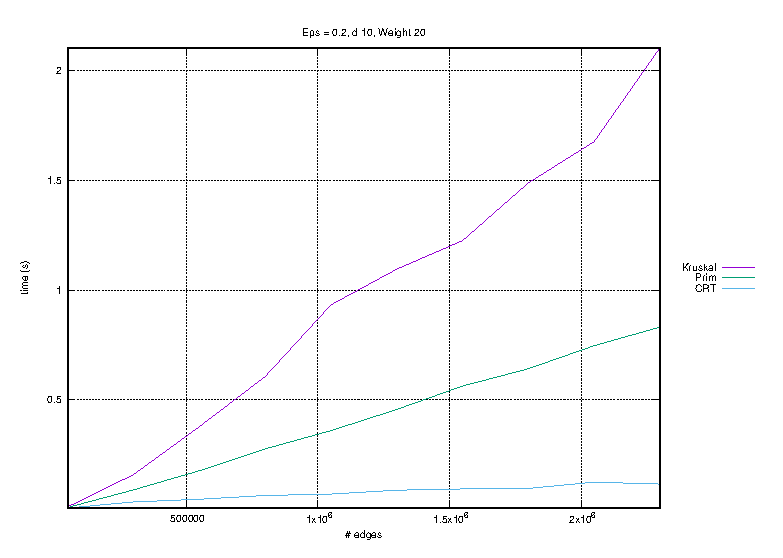
\includegraphics[scale=0.6]{GAUSSIAN_E_02_W_20_D_10_EPS}
  \caption{Gaussian}
\label{GAUSSIAN_E_02_W_20_D_10}
 \end{figure}


\begin{figure}[htbp]
  \centering 
  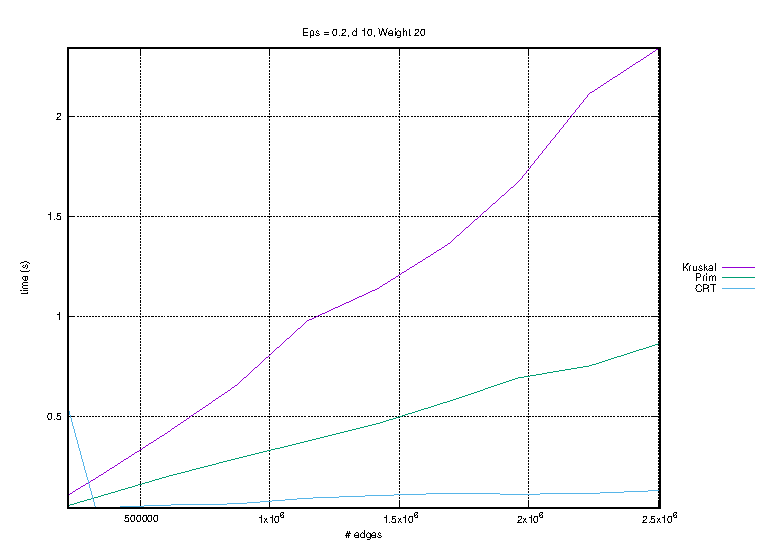
\includegraphics[scale=0.6]{SCALE_FREE_E_02_W_20_D_10_EPS}
  \caption{Scale-Free}
  \label{SCALE_FREE_E_02_W_20_D_10}
  \end{figure}

  
  \begin{figure}[htbp]
  \centering
   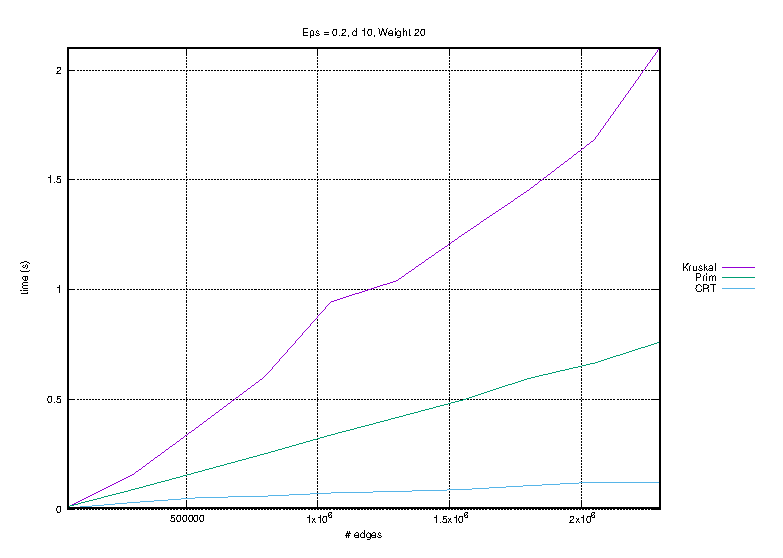
\includegraphics[scale=0.6]{SMALL_WORLD_E_02_W_20_D_10_EPS}
  \caption{Small-World}
  \label{SMALL_WORLD_E_02_W_20_D_10}
  \end{figure}

  
  \begin{figure}[htbp]
  \centering
   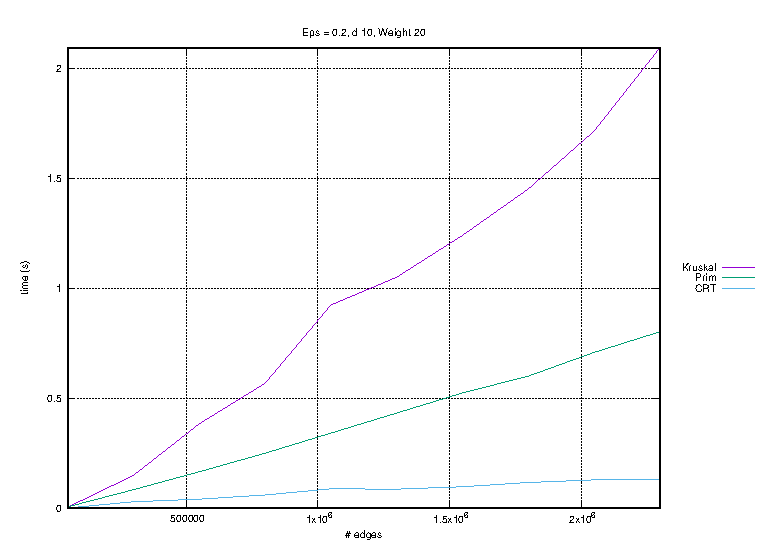
\includegraphics[scale=0.6]{UNIFORM_E_02_W_20_D_10_EPS}
  \caption{Uniform}
  \label{UNIFORM_E_02_W_20_D_10}
  \end{figure}
  
At first, we can observe that given fixed values of $d$, $w$ and $\varepsilon$ the CRT Algorithm respects the sub-linearity property, for all the different types of graphs in our dataset, as the reader can see in the figures from~\ref{GAUSSIAN_E_02_W_20_D_10} to~\ref{UNIFORM_E_02_W_20_D_10}.\\

Now we want to see what happens if there is an increase in the value of $d$, keeping other values unchanged.

  \begin{figure}[htbp]
  \centering
   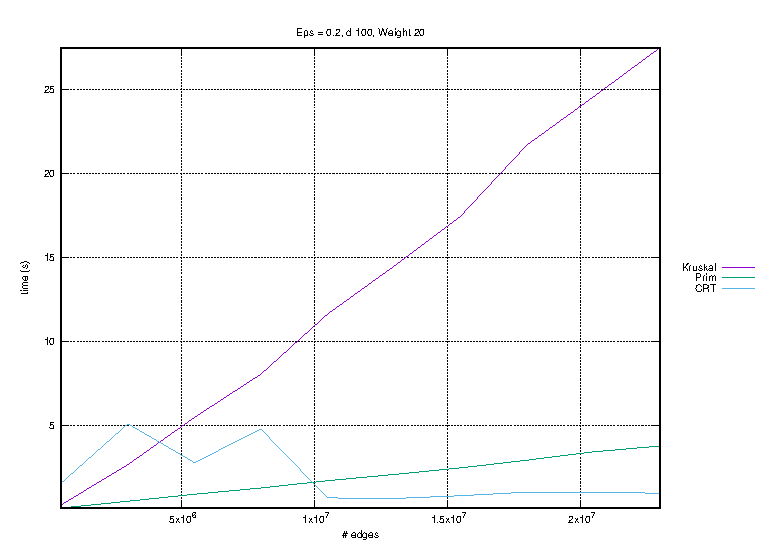
\includegraphics[scale=0.6]{GAUSSIAN_E_02_W_20_D_100_EPS}
  \caption{Gaussian}
  \label{GAUSSIAN_E_02_W_20_D_100}
  \end{figure}

  
   \begin{figure}[htbp]
  \centering
   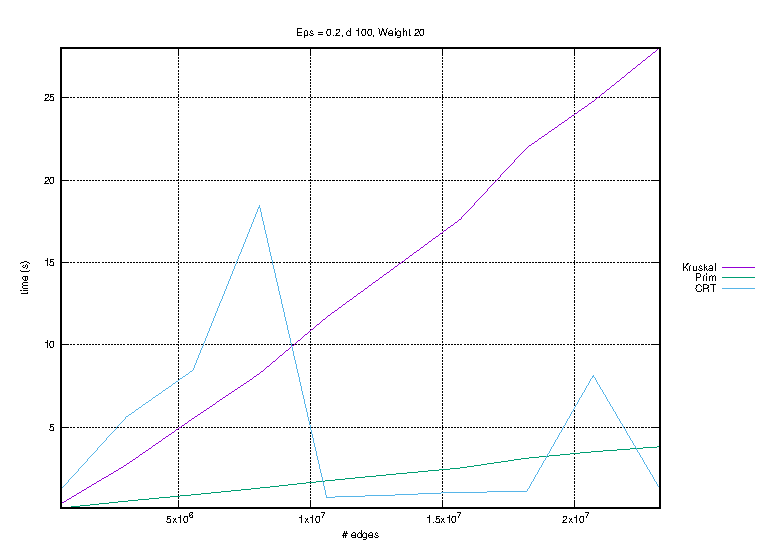
\includegraphics[scale=0.6]{SCALE_FREE_E_02_W_20_D_100_EPS}
  \caption{Scale-Free}
  \label{SCALE_FREE_E_02_W_20_D_100}
  \end{figure}
 
 
While in the corresponding Small-World graph and the corresponding Uniform graph the trend is similar to the Gaussian graph (Fig.~\ref{GAUSSIAN_E_02_W_20_D_100}), in the Scale-Free case the reader can easily see that CRT algorithm takes a little 'more time' to down permanently under Prim execution time (Fig.~\ref{SCALE_FREE_E_02_W_20_D_100}). This can be related to the presence, in this kind of graph, of different nodes that have an high degree, which can make slower the execution. \\ The reader can also may notice that for small instances (few edges) the CRT algorithm is worse than deterministic algorithms, but when increasing the graph size the trend returns to be sub-linear again. \\Also comparing, for example, (Fig.~\ref{GAUSSIAN_E_02_W_20_D_100}) with the corresponding (Fig.~\ref{GAUSSIAN_E_02_W_20_D_10}), one can easily see that the performances become worse, as expected having increased the $d$ value. \\ 

Let us now see what happens if we increase $w$, keeping $d$ and $\varepsilon$ unchanged.
 
\begin{figure}[htbp]
  \centering
   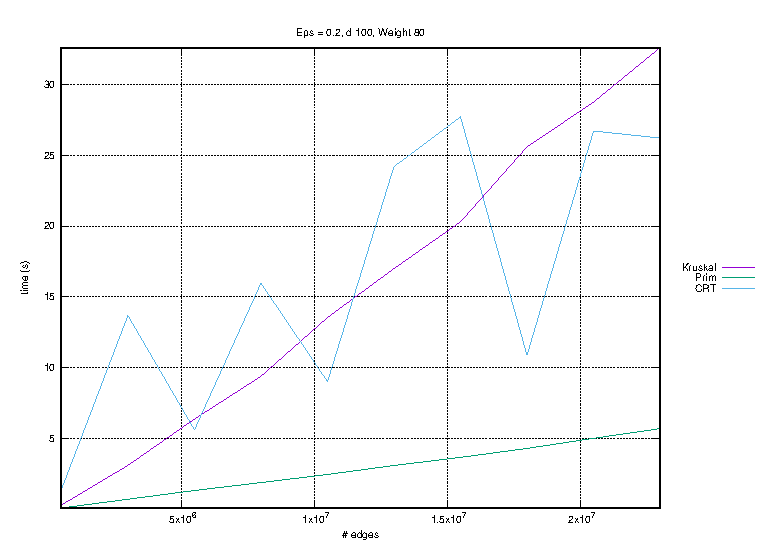
\includegraphics[scale=0.6]{GAUSSIAN_E_02_W_80_D_100_EPS}
  \caption{Gaussian}
  \label{GAUSSIAN_E_02_W_80_D_100}
  \end{figure}
  
  \begin{figure}[htbp]
  \centering
   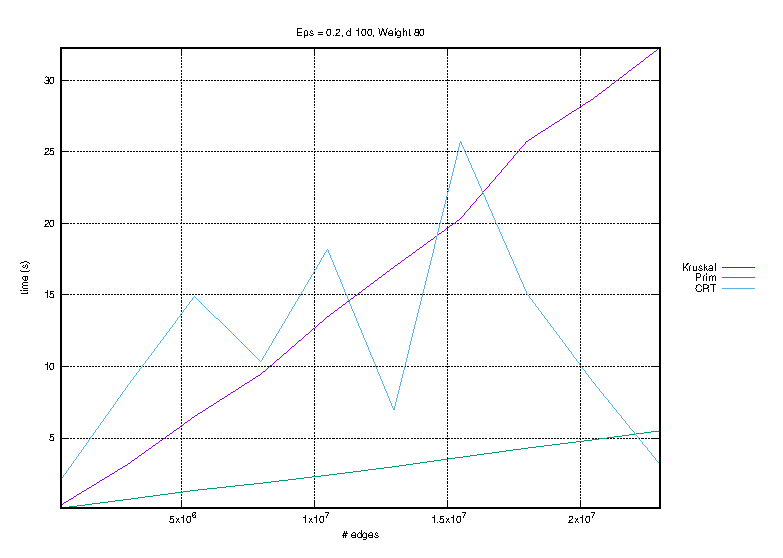
\includegraphics[scale=0.6]{SMALL_WORLD_E_02_W_80_D_100_EPS}
  \caption{Small-World}
  \label{SMALL_WORLD_E_02_W_80_D_100}
  \end{figure} 
 
As expected, the CRT running time is higher than before. To be precise, what happens is that for the Gaussian, for the Scale-Free and for the Uniform the trend is about the same (Fig.~\ref{GAUSSIAN_E_02_W_80_D_100}), while for the Small-World case the reader can observe (Fig.~\ref{SMALL_WORLD_E_02_W_80_D_100}) that for large graph instances the trend becomes sublinear. We can imagine that the same happens for even larger instances also in the previous three kinds of graph.
 
To see if this is true we create an ad-hoc graphs dataset, that is an extension of our previously discussed dataset.\\
We generate an extension in the Uniform graphs dataset, adding larger instances (i.e. in terms of nodes and edges), and we want to see if the CRT algorithm becomes sub-linear, as expected, onwards from a certain point.

\begin{figure}[htbp]
  \centering
   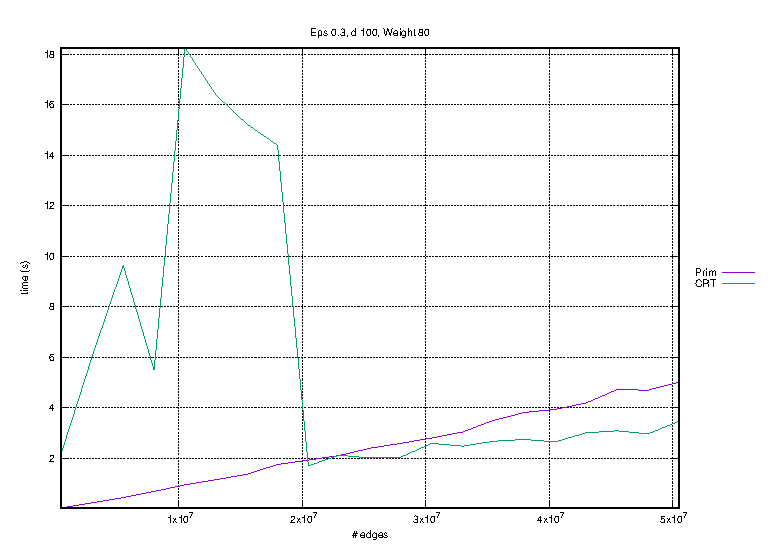
\includegraphics[scale=0.6]{UNIFORM_BIG_RUN_EPS}
  \caption{Uniform}
  \label{UNIFORM_BIG_RUN_EPS}
  \end{figure} 
 

As the reader can see in Fig.~\ref{UNIFORM_BIG_RUN_EPS}, for larger instances the CRT algorithm really becomes sub-linear and its performances are better than, for example, Prim Algorithm.
\\

This is in agreement with the definition of the $O$ notation, that, for large arguments, indicates that the asymptotic behavior is of a certain type.\\

To conclude the discussion on the consistency of the execution time, we want now to see what happens in the case we increase $\varepsilon$, keeping $d$ and $w$ unchanged. \\Since the $\varepsilon$ parameter is a denominator for the estimated running time, what is expected is that an increase of this value corresponds to improved performances.

We can compare, for example, the performances of the CRT algorithm on two Small-World graphs with the following parameters: 
\begin{itemize}
\item $d=10$ 
\item $w=20$
\item and compare what happens for $\varepsilon=0.2$ and $\varepsilon=0.4$
\end{itemize}
 

 \begin{figure}[htbp]
  \centering
   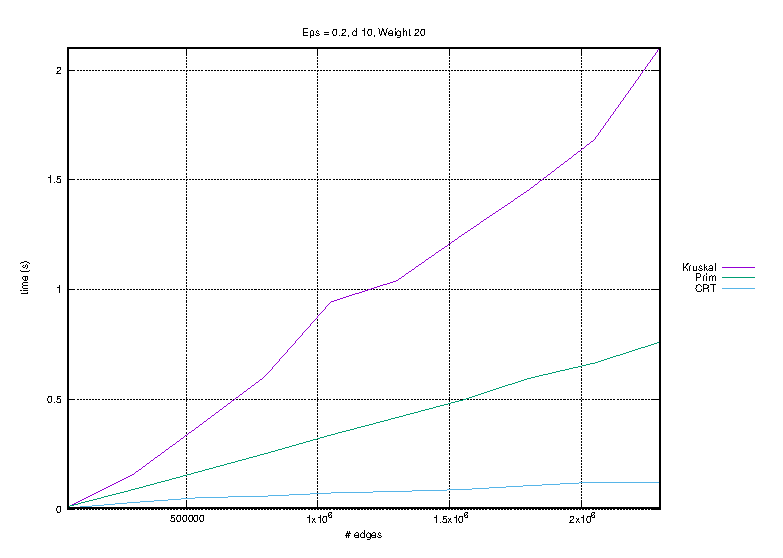
\includegraphics[scale=0.6]{SMALL_WORLD_E_02_W_20_D_10_EPS}
  \caption{Small-World, $\varepsilon=0.2$}
  \label{SMALL_WORLD_E_02_W_20_D_10_second}
  \end{figure}

  \begin{figure}[htbp]
  \centering
   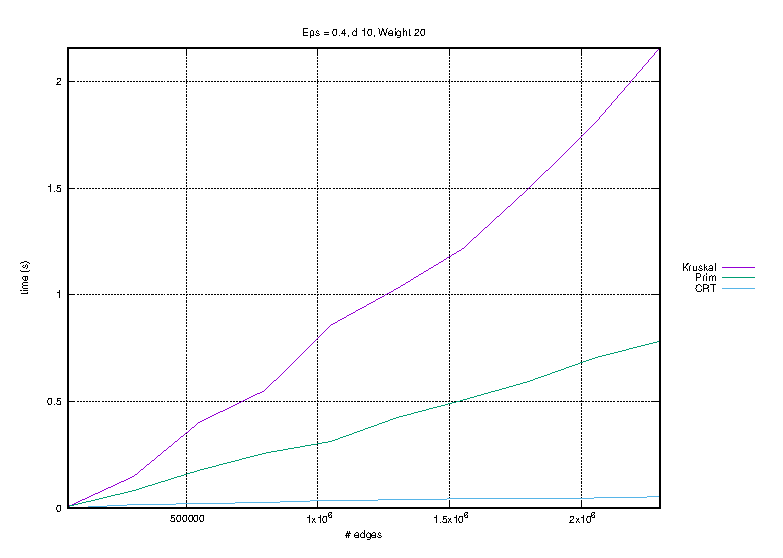
\includegraphics[scale=0.6]{SMALL_WORLD_E_04_W_20_D_10_EPS}
  \caption{Small-World, $\varepsilon=0.4$}
  \label{SMALL_WORLD_E_04_W_20_D_10}
  \end{figure}
 
 
 
 
The reader can easily see that the CRT trend has decreased.
 
 
 
 \section{Final thoughts} 
 
As expected, a probabilistic algorithm like the CRT allows us to compute an approximation of the Minimum Spanning Tree in sublinear time on the number of edges, under certain conditions.\\ Tunable parameters, that depends on $\varepsilon$, allows us to perform either a better or a worse approximation, implying respectively a very slow and a very fast computation. The choice of a small value of $\varepsilon$ can lead to terrible running times, and for these values it does not make sense to compare the CRT algorithm with any other deterministic algorithm.\\
For other $\varepsilon$ values, instead, we prove the good performances of the CRT. The reader can easily view the better performances of CRT algorithm versus Prim algorithm or Kruskal algorithm watching the line charts in the previous section of this paper.
 
 
 
 
 
 
 
\begin{thebibliography}{10} 
\bibitem{crt} {\sc B. Chazelle, R. Rubinfeld, and L. Trevisan},Approximating the minimum spanning tree weight in
sublinear time. SIAM J {\em Computing}, 34, 2005.


\end{thebibliography} 

\end{document} 

